\documentclass[aspectratio=169,xcolor=dvipsnames,UTF8]{beamer}
\usetheme{SimplePlus}

\usepackage{ctex}
\usepackage{CJK}
\usepackage{fontspec}
\usepackage{listings}
\usepackage{listings-ext}
\usepackage{color}
\usepackage{hyperref}
\usepackage{subfigure}
\usepackage{graphicx} % Allows including images
\usepackage{booktabs} % Allows the use of \toprule, \midrule and \bottomrule in tables
\usepackage{caption}
\usepackage{indentfirst}

% -- 压制警告可选
%\PassOptionsToPackage{quiet}{xeCJK}

%图目录配置
\graphicspath{{images/}}
%图注解配置
\captionsetup{font={tiny}}
%----------------------------------------------------------------------------------------
%	标题页
%----------------------------------------------------------------------------------------

% 标题
\title[Web常见问题指北]{Web常见问题指北} 
\subtitle{浏览器同源策略及常见云产品涉及跨域问题和解决方法}

\author[Wei-Zhao] {Wei-Zhao}

\institute[Anchnet] 
{
    Anchen.Net
}
% 按编译日期计
\date{\today}


\begin{document}

%----------------------------------------------------------------------------------------
% 标题页
%----------------------------------------------------------------------------------------
\begin{frame}
    \titlepage
\end{frame}
%----------------------------------------------------------------------------------------


%----------------------------------------------------------------------------------------
% 目录页
%----------------------------------------------------------------------------------------
\begin{frame}{目录}
    \tableofcontents
\end{frame}
%----------------------------------------------------------------------------------------



%------------------------------------------------
\section{引言}
%------------------------------------------------
\begin{frame}{引言-跨域报错}

	\begin{figure}
		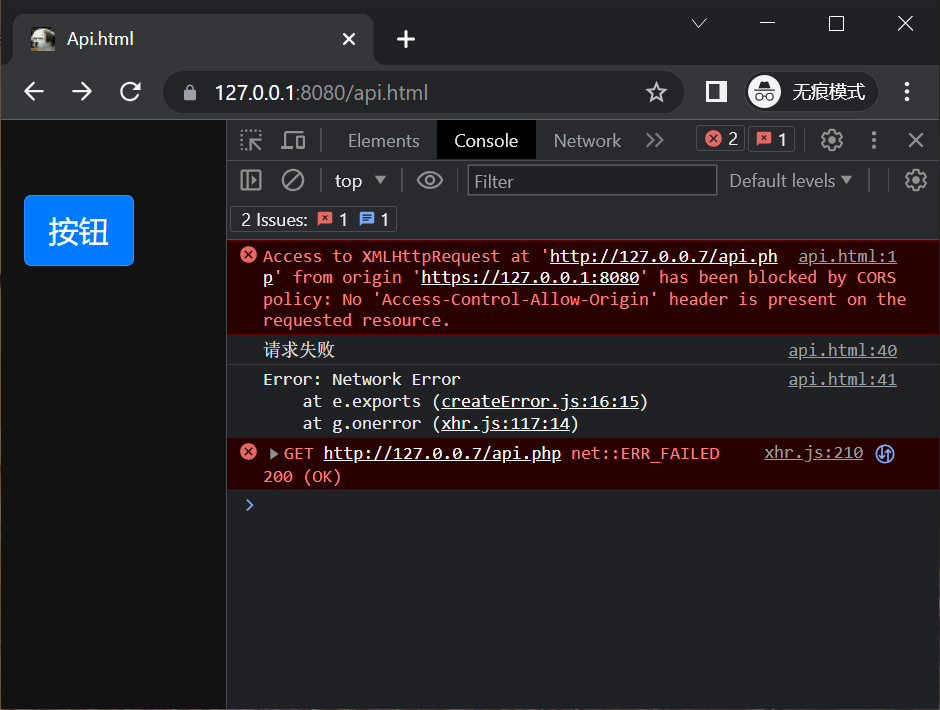
\includegraphics[width=0.48\linewidth]{cors-console-error.png.eps}
		%\caption{ \fontsize{0.5pt}{0pt} 1.1 Chrome控制台错误}
		%\begin{center}
		%	 1.1 Chrome控制台错误
		%\end{center}
		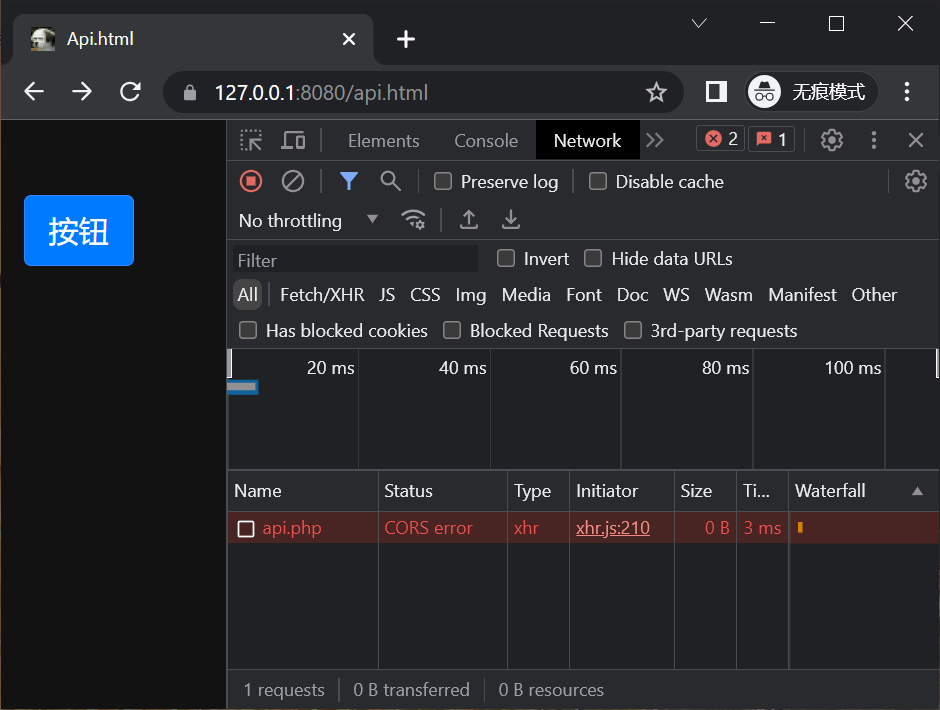
\includegraphics[width=0.48\linewidth]{cors-network-error.png.eps}
		%\caption{ \fontsize{0.5pt}{0pt} 1.2 Chrome控制台网络}
		%\begin{center}
		%	 1.2 Chrome控制台网络
		%\end{center}
	\end{figure}

%{\songti 宋体}	
%{\heiti 黑体}
%{\fangsong 仿宋}
%{\kaishu 楷书}
\end{frame}

%------------------------------------------------
\section{同源策略}
%------------------------------------------------
\begin{frame}{同源策略(Same Origin Policy)}
	\begin{block}{}
			\emph{浏览器的同源策略,限制了来自不同源的“document”或脚本,对当前“document”读取或设置某些属性。}
	\end{block}
	\vspace{2em}
\setlength{\parindent}{2em}同源策略(Same Origin Policy)是一种约定,它是浏览器最核心也最基本的安全功能,如果缺少了同源策略,则浏览器的正常功能可能都会受到影响。可以说Web是构建在同源策略的基础之上的,浏览器只是针对同源策略的一种实现。
	
\end{frame}


%------------------------------------------------
\section{如何解决跨域报错}
%------------------------------------------------
\begin{frame}
 3
\end{frame}

%----------------------------------------------------------------------------------------
% 结束页
%----------------------------------------------------------------------------------------

\begin{frame}
    \Huge{\centerline{\textbf{谢谢观看}}}
\end{frame}

%----------------------------------------------------------------------------------------

\end{document}